


%%%% 1. DOCUMENTCLASS %%%%
\documentclass[journal=tosc,final]{iacrtrans}
%%%% NOTES:
% - Change "journal=tosc" to "journal=tches" if needed
% - Change "submission" to "final" for final version
% - Add "spthm" for LNCS-like theorems


%%%% 2. PACKAGES %%%%
\usepackage{graphicx}
\usepackage{framed} 
\usepackage{xcolor}
\usepackage{tcolorbox}
\usepackage{xcolor} 
\colorlet{shadecolor}{gray!25}
\definecolor{mshadecolor}{rgb}{0.7421875,0.7421875,0.7421875}
%%%% 3. AUTHOR, INSTITUTE %%%%
\author{Moritz Rupp}
\institute{
  Hochschule Albstadt-Sigmaringen, Albstadt, Germany, \email{ruppmori@hs-albsig.de}
  
}
%%%% NOTES:
% - We need a city name for indexation purpose, even if it is redundant
%   (eg: University of Atlantis, Atlantis, Atlantis)
% - \inst{} can be omitted if there is a single institute,
%   or exactly one institute per author


%%%% 4. TITLE %%%%
\title{Fuzzing Methods}

\author{Moritz Rupp}
%%%% NOTES:
% - If the title is too long, or includes special macro, please
%   provide a "running title" as optional argument: \title[Short]{Long}
% - You can provide an optional subtitle with \subtitle.

\begin{document}

\maketitle
\author


%%% 5. KEYWORDS %%%%
\keywords{Offensive Security \and Fuzzing \and Brute-Forcing \and It-Security \and Testing }


%%%% 6. ABSTRACT %%%%
\begin{abstract}
Software testing has become a ever more important security method. Since modern Software becomes increasingly complex it's not possible to rely fully on manuel static testing. Fuzzing is a dynamic automated way of testing and sees growing usage among security proffesionals. This paper examines different apporaches to use this technologys. 
\end{abstract}
\tableofcontents
\newpage

%%%% 7. PAPER CONTENT %%%%
\section{Introduction}
Development of any kind has always come with bugs, errors and unintentionally behaviour. Software is no exception. Increasingly complex programs and growing technology stacks contribute to this problem. On top of that, finished components are often continuously integrated. As a result, it becomes ever more difficult to predict final program behaviour. This yields in risks, particular if an application is processing external data input. If not handled correctly it can pose security vulnerabilitys or data breaches. The bigger a programm gets, more often such unwanted appearances occur. A field in which this is most noticable is web-development. Whereas 10 years ago, most websites were built with the help of one or two technologys, modern web-applications often use several framework with huge amounts of dependencys. This lead to an increasing amount of security bugs. Different approaches in software testing tries to oppose that development. Back when software was relativly simple and free of dependencys, manuel testing was the state of play. That included code reviews and manuel checks for potentiell exploitation. This was time consuming and needed experts for every specific application. Therefore static analyis was quickly adapted. This contained new techniques such as pattern search with a control flow graph, data dependency graph and data flow analysis. When software grew even more in complexity, security researchers needed a more scalable approach. Hence dynamic analyis was implemented. This method tries to understand software behaviour by inputing different types of data. Fuzz-testing is the cutting edge of this technique and will be explored in this paper. At first we will examine the basic concept and functionality. Following different methods in Fuzzing will be explored. Finally we will have a conclusion that covers the pros and cons of Fuzz-testing. 
\section{What is Fuzzing?}
Fuzz testing or fuzzing is a method of testing software to detect security holes in applications, operating systems, and networks. It involves flooding their input interfaces with random data, called fuzz, to make them crash or trigger unexpected programm behaviour.\footnote{Source 1} Furthermore the computation results are monitered and reported, all in an automated way. Fuzzing has become increasingly more relevant among security researchers and is used by almost all big tech companys for penetration testing. Tech leaders find more than 80\% of their bugs by using different fuzzing Methods.\footnote{Source 2} Google for example  has found over 19 thousend errors in their browser projekt chrome.\footnote{Source 3} Microsoft used dynamic analysis to test one of their flagship projects 'office' and found nearly 2000 bugs using the fuzzing tool afl. Also open source project such linux use Fuzzing methods on a great scale. Many security bugs within the Linux Kernel have been found this way.\\
Generally a distinction can be made on how fuzzing is executed on a specific interface. Depending on the application or infrastructure of the target system, different types of fuzzers can be used. Application Fuzzing will approach a system by testing functionalitys such as buttons, input fields or command line parameters. File format fuzzing tries to generate corrupted files and feed them to the corresponding target for processing. Other types of Fuzzing targets include Protocol Fuzzing and Network fuzzing.\\
In addition more distinction can be made on how the fuzzing inputs or test cases are generated. There are two approaches. Mutation based Fuzzers alter existing data samples to create new test cases. Generation-Based Fuzzers define new data based on the expected input of the target specification. Both methods have pro and cons and will be covered in more details later on.
\newpage
\section{Functionality}
This section will provide a perspective on the basic concept of Fuzzing. Regardless of the specific implementation, the core process of all fuzzers remains the same. First the target interface has to be identfied. Relevant are all interfaces that allow external data input. This ranges from network sockets, user-input on a website to linux binarys et cetera. Specifally interesting are interfaces that are reachable by unpriviliged users. The act of finding those target interfaces highly depends on the tested application and could include things like code reviews or portscanning. Based on the findings, the fuzzer input can now be generated. This is one main task of the actuall fuzz-engine. In the most basic case, it will generate pseudo random inputs based of the given seed. The seed could contain anything that makes sense in the context of the expected data, essentially a snapshoot of valid inputs for the target system. Mostly combinations of strings and intergers. Following the test cases can be passed to the  target system. Depending on the identfied interfaces, different transfer methods are used. This could involve HTTP Requests, tcp sockets or simply files as input parameters for a programm. While the Fuzz-eingine is sending the generated inputs, the target system has to be monitered to track how the testcases effect the system behaviour. Monitering and tracking can be achieved with different approaches. A convinient but not always available case are logging functions of the target system. They can be simply read out during or after the fuzzing process. If the target is lacking such functionalitys it is neccecarry to implement feedback instrumentations. Those are compile time binarys that are inserted into the target code to track and tell the fuzzer which parts of the internal programmflow is effected. This ensures to establish a correlation between test cases and programm behaviour. The Feedback gets send back to the fuzzing-engine and can be reprocessed.
\begin{shaded}

\begin{center}
 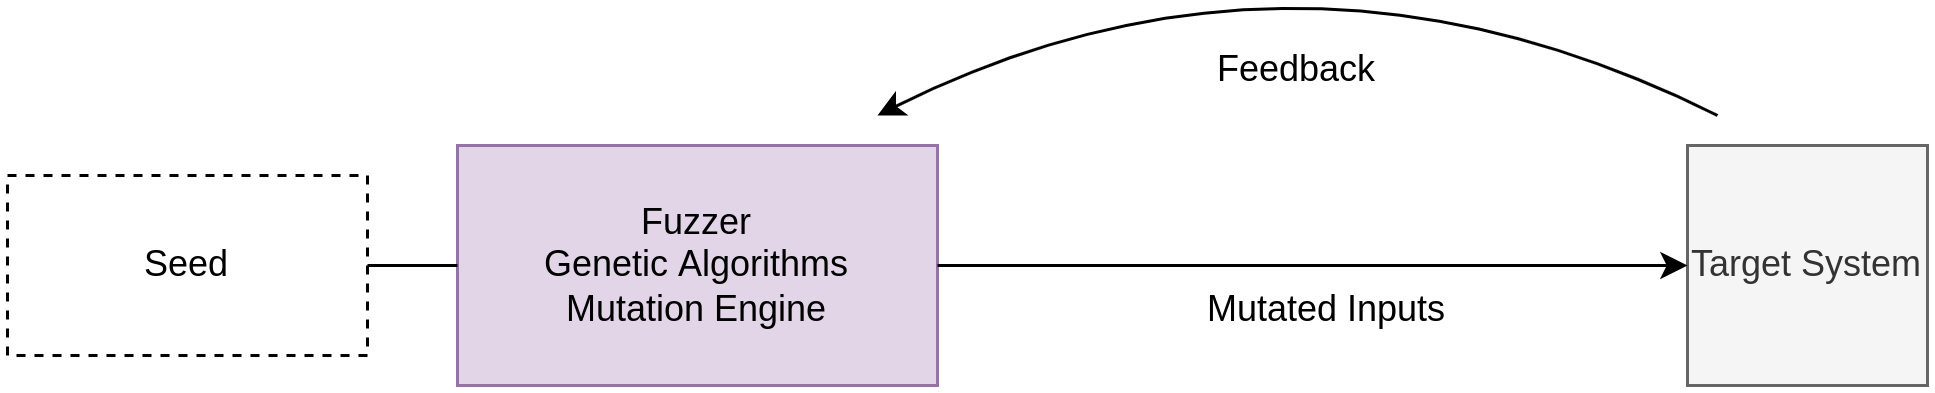
\includegraphics[scale=0.2]{../final2.png}
 \end{center}
\begin{center}

 Figure 1: Basic Fuzzing application\footnote{source n}
\end{center}
\end{shaded}
\noindent Figure 1 provides an overview of a basic mutation based fuzzing implementation. The Fuzzer as seen between the Seed and the target system includes a mutation engine and genetic algorithms.\footnote{source 1} The Fuzzing process can now lapse as follows.\\
The Seed streams valid inputs to the fuzzer that will modifiy these with the help of the mutation engine. Following the mutated inputs gets send to the target system in which feedback instrumentations listen for exceptions, log them and provide feedback to the fuzzer. Based on that genetic algorithms produce further inputs. Once the fuzzing process has endet, it is now possible to analyse and minimize the findings. This includes to determine if a tracked exeption could actually cause a vulnability or even an exploit. Furthermore these assessments are rated. This is done by ranking frameworks like the common vulnability scoring system(CVSS). Finally all relevant informations are summed up, reported and passed to the corresponding responsible. 



\newpage
\section{Fuzzing Methods}
Due to the huge target landscape, enourmes classifications exist around fuzzing. In this section we will further examine the different input types such as mutation and generation based fuzzers.
\subsection{Mutation based fuzzing}
Called dumb fuzzers since they only alter already existing data \dots
\subsection{Generation based fuzzing}
Smart Fuzzers, since they generate data from the go\dots
\newpage
\subsection{Application Fuzzing}

\subsection{Protocoll Fuzzing}
\subsection{File format Fuzzing}
\subsection{Network Fuzzing}
\newpage
\section{Tooling}
Hundrets of fuzzing tools are available. Like wfzuu, afl and zfuzz etc..
\subsection{Practical example}
We will fuzz a webserver with afl\dots
\section{Conclusion}



%%%% 8. BILBIOGRAPHY %%%%
\bibliographystyle{alpha}
\bibliography{abbrev3,crypto,biblio}
%%%% NOTES
% - Download abbrev3.bib and crypto.bib from https://cryptobib.di.ens.fr/
% - Use bilbio.bib for additional references not in the cryptobib database.
%   If possible, take them from DBLP.

\end{document}
